%****************************************************
%	CHAPTER 1 - INTRODUCTION
%****************************************************
\chapter{Introduction}
\label{ch:intro}
%====================================================
\section{Foreword}
\label{sec:intro.foreword}
%====================================================
\subsection{A Brief Background to the Study}
\label{subsec:intro.foreword.background}
%====================================================
A popular topic for current control and automation research is that of quadrotor UAVs. Attitude control of a quadrotor poses a unique 6-DOF control problem, to be solved with an under-actuated 4-DOF system. As a result the $\phi$ pitch and $\theta$ roll plants aren't directly controllable. The attitude plant is often simplified around a stable operating point. The trimmed operating region is always at the inertial frame's origin; resulting in a zero-set point tracking problem. The highly coupled non-linear dynamics of a rigid body's transnational and angular motions arise from gyroscopic torques [Section:~\ref{subsec:dynamics.nonlinearities.gyrotorques}] and Coriolis accelerations [Section:~\ref{subsec:dynamics.nonlinearities.coriolis}]. These effects are negligible around the origin, hence the origin trim point removes the system's nonlinearities. The control system can then reduce\footnote{Expanded upon in Appendix:\ref{app:stddynamics}} each state variable, $\vec{X}_b=\big[\phi~\theta~\psi~x~y~z\big]^T$, to individual SISO plants.
\par
As almost every recent quadrotor research paper mentions, the late interest in the platform is from recent emergences in availability of MEMS systems and low-cost microprocessors. Such advancements accomodate onboard state estimation and control algorithm processing in real time. Developmental progress in quadrotors and, to a lesser extent, UAVs in general has led to rapidly growing enthusiast communities. HobbyKing\cite{hobbyking} is now synonymous with providing custom DIY hobbyist quadrotor kits, no longer just a reailter for prebuilt commercial products like the DJI Phantom\cite{phantom}.
\par
The avenue for potential application of both fixed wing and VTOL UAVs is expansive, supporting civil\cite{civilquadcopter}, agricultural\cite{agriculturequadcopter} and security\cite{videosurveillancequadcopter} industries. The quadrotor platform provides a mechanically simple platform on which to test advanced aerospace control algorithms. Commercial drone usage in industry is already emerging as a prolific sector; especially in Southern Africa. Subsequently following the $8^{th}$ amendment of civil aviation laws \cite{dronelaw}, commercial use of UAVs has been both legalized and regulated. Research into any non-trivial aspect of the field will therefore be to extremely valuable to the field as a whole. 
\par
Large scale quadrotor, hexrotor and even octorotor UAVs are popular intermediate choices for aerial cinematography due to their high payload capacity.  The cost of a commercial drone like the SteadiDrone Maverik \cite{steadidrone} is far less than a chartered helicopter used for the same panoramic aerial scenes or on-site inspections. One foreseeable issue which may hinder commercial drone progress in the agricultural and civil sectors is the consequential inertial effects from scaling up the aerospace bodies. When scaling up any vehicle, its performance is adversely affected if actuation rates aren't proportionately increased.
%====================================================
\subsection{Research Questions \& Hypotheses}
\label{subsec:intro.foreword.hypotheses}
%====================================================
The difficulty with quadrotor control is that fundamentally it's unstable and under-actuated, \emph{empirically proven later with Layupanov Theorem in Chapter:\ref{ch:control}}. A quadrotor has only four controllable inputs, namely propeller rotational speeds, $\Omega_{1,2,3,4}$, which are then abstracted\footnote{The abstraction of which is explored in Appendix:\ref{app:stddynamics}} to virtual control inputs net torque, $\vec{\tau}_{net}=[\tau_{\phi}~\tau_{\theta}~\tau_{\psi}]^T$, and a perpendicular heave thrust $\vec{T}_{net}=\sum_{i=1}^{4}~T(\Omega_i)$. Those four inputs have to affect both the linear X-Y-Z positions, $\mathcal{E}=[x~y~z]^T$, and angular pitch, roll and yaw rotations, $\eta=[\phi~\theta~\psi]^T$. Pitch and roll torques, $\tau_{\phi}$ \& $\tau_{\theta}$, are induced from differentials thrusts of each opposing propeller. Yaw torque, $\tau_{\psi}$, is dependent on net aerodynamic torque about the rotational axes of each propeller (See Section:\ref{subsec:dynamics.aero.bem}). Aerodynamic responses are non-linear and fluctuating sources of control torques and as such the body's yaw control is depreciated. A result of the under-actuation is that the attitude control problem then becomes a zero set point problem, any other attempt to track attitude is ill-posed.
\par
The aim of this project is to implement quadrotor attitude and position set point tracking by solving the problem of its inherent under-actuation. Inspired by Boeing/Bell Helicopter's V22 Osprey and the tilting articulation of its propellers, the prototype design proposed here introduces two additional actuators for each of the quadrotor's lift propellers. Specifically, adding rotations about the $\hat{X}$ and $\hat{Y}$ axes for each motor/propeller pair. The resultant is a vectored 3 dimensional thrust force rather than a bound perpendicular heave thrust. The control problem is then posed as the design and allocation of net forces, $\vec{F}_{net} = [F_x\;F_y\;F_z]^T$, and torques, $\vec{\tau}_{net} = [\tau_{\phi}~\tau_{\theta}~\tau_{\psi}]^T$, for a general 6-DOF body such that for any given trajectory, $X_d(t)=[x~y~z~\psi~\theta~\phi]^T$, the error state $X_e(t) = X_d(t) - X_b(t)$ asymptotically tends to $\vec{0}$.
\begin{equation} \label{eq:trajectoryerror}
lim_{t \rightarrow \infty} X_e(t) = \vec{0}\hspace{10pt}\forall X \in \mathbb{R}^n
\end{equation}
Where $n$ is the degree of freedom the system has. The over-actuation brings about the need for a control allocation scheme which distributes the 6 commanded system inputs (net torques and forces) among the actuator set (12 actuators) in order to optimize some objective function secondary to that of Eq:\ref{eq:trajectoryerror}. The potential improvement(s) for exploiting those over-actuated elements is the most novel outcome that this project will yield. A cost function aimed at optimizing some aspect unique to aerospace bodies is going to be a completely unique contribution.
\par
Part of the control research question is the multivariable treatment of the system, making no assumptions or simplifications to the non-linear dynamics involved in the quadrotors motion and its operational conditions. Standard linearizations applied to the quadrotor's control plant won't hold true for the more aggressive manoeuvres; they're dependent on small angle approximations and negligible 2$^{nd}$ order effects. A stabilizing control law solution will need to expand and simulate the existing kinematic model of an aerial body and apply it to a quadrotor's motion. Following this there must be design, development and control of the new actuator suite which is to be implemented on a quadrotor platform. Final key outcomes for the project are the simulation analysis and prototype construction for the proposed design and the conclusion drawn thereon.
\par
Introducing relative motion within an unconstrained body will produce a lot of unwanted dynamics like inertial and gyroscopic responses, amongst others. A rotating propeller will respond to pitching much like a Control Moment Gyroscope \cite{cmg} or a flywheel, producing a precipitation torque. A less trivial aspect to consider is the aerodynamic torque produced from the propeller's aerofoil profile. Such induced responses occur in planes perpendicular to whatever the propeller's rotation exists in. These aspects aren't normally compensated for due to a quadrotor's fundamental co-planar propeller rotation. It's anticipated that a plant dependent control solution will have to compensate for these dynamics, which if left unaccounted for could potentially cause instability.
%====================================================
\subsection{Significance of Study}
\label{subsec:intro.foreword.significance}
%====================================================
Due to the huge popularity of quadrotor platforms as research tools, any work that expands the UAV \& quadrotor general body of knowledge will prove to be valuable. With that being said, there is already a vast amount of existing research on linear and non-linear control techniques for regular quadrotor platforms. The attitude loop is the most common topic for control research, requiring an under-actuated solution and mostly linearized around the origin (See Appendix:\ref{app:stddynamics}). Far less common is the application of optimal flight path and trajectory planning to quadrotor control. The uniqueness and difficulty of the quadrotor attitude control does not hold true for its position control, so standard techniques can be used for way point planning and the like once the attitude control problem has been answered.
\par
The most significant aspect of this project is the attitude control, discussed later in Section:\ref{sec:control.attitude}. The over-actuation of the proposed design and, more critically, the manner in which the controller's (virtual) output is distributed among those control effectors would appear to be the first of its kind. Otherwise known as control allocation, the requirements of the distribution algorithm(s) are outlined in Section:\ref{sec:control.allocation}. Dynamic set point attitude control for aerospace bodies is not a subject heavily researched outside the field of satellite attitude control. Even papers which propose similarly complicated mechanical over-actuation (expanded upon in next in the literature review, Section:\ref{sec:intro.litreview}) hardly broach the topic of tracking attitude set points away from the origin.
\par
Whilst the control plant (developed in Chapter:\ref{ch:control}) does indeed close both the position and attitude control loops, there is no consideration of trajectory generation nor flight path planning. Such topics are well discussed elsewhere in a far more concise and deliberate way than this project could ever hope to achieve. Once closed loop position and attitude control have been achieved, the control algorithms can be adjusted to account for higher order state derivative (acceleration, jerk and jounce) tracking needed for nodal way point planning. The heuristics involved with flight path planning are well documented and their implementation is a relatively academic task.
\par
Where possible the system identification and control (design and allocation) for this project is kept both modular and generically applicable. The intention here is that its pertinence falls not only within the UAV field but to any aerospace or free body attitude control. Hopefully this investigation can be expanded upon with more in-depth research on one of the subsystems without compromising the stability of the whole plant. Provisionally, an obvious outcome which the investigation could yield is improved yaw control of a quadcopter's attitude. However, if the express purpose was just to improve yaw control, it could be done with a dramatically less complicated design.
\par
Furthermore, the project could provide greater insight into high bandwidth actuation and thus a faster control response for larger aerospace bodies. Any standard quadrotor uses differential thrust to develop a torque about its body. Such actuation suffers a second order inertial response when the propellers accelerate or decelerate, $\tau_{simplified}=\mathbb{I}_f~\dot{\omega}_{i}$. Prioritizing pitching the propeller's principle axis of rotation rather than changing the propeller's speed could potentially improve the virtual control response. This is entirely dependent on how the allocator block is prioritized (presented in Section:\ref{sec:control.allocation}). The exact effects of different actuator prioritization and distribution in the context of aerospace control are wholly unique to this dissertation.
%====================================================
\subsection{Scope and Limitations}
\label{subsec:intro.foreword.scopeandlim}
%====================================================
\subsubsection{Scope}
\label{subsubsec:intro.foreword.scope}
%====================================================
Critical to this project is the conceptualized design and prototyping of a novel actuation suite to be used on a quadrotor platform. The express purpose of which is to apply dynamic set point attitude control to the body. Stemming from this is an investigation into the kinematics that are potentially influenced by the design and the structure's relative motion. In order to apply correct control theory to achieve the attitude tracking on a physical prototype, the plant dynamics must first be identified for input responses to be approximated with confidence. Aspects of the mechanical design are covered next in Section:\ref{sec:proto.design} but, beyond the cursory investigation, there is no scope for materials analysis or stress testing of the design. To the detriment of the project, the design will either produce an over-engineered or catastrophically under-engineered solution. The scope focuses mainly on the control application and embedded systems design, not the structural integrity of a proposed frame given the forces it may undergo. Physical measurements are only made for critical kinematics, such as inertial measurements for the second order gyroscopic and inertial dynamic responses.
\par
As mentioned in the antecedent Section:\ref{subsec:intro.foreword.significance}, trajectory \& flight path planning are not ubiquitous with this dissertation. Derivations for the differential equations which dictate a 6-DOF body's movement are wholly applicable to any dynamic (rigid or otherwise) aerospace body, although some particular standards are used (sic Z-Y-X Euler Aerospace Sequence, Section:\ref{sec:proto.conventions}). Similarly the control plant is stabilized with non-linear state space control techniques, aided and justified by Lyupanov theorem. Alternative solutions using Model Predictive Control or Quantitative Feedback Theory could provide more refined or effective controllers, however they aren't presented and remain open to further investigation. Quadrotor attitude control is commonly stabilized with feedback linearizations, decoupling the plant around a trim point so that SISO techniques can be applied. A derivation of such a linearization is included in Appendix:\ref{app:stddynamics} but beyond that there are no further discussions. Any comparison between non-zero and zero-set point attitude control of quadrotor is difficult as the fundamental objectives are in stark contrast with one another.
\par
Arguably the most important and indeed novel aspect of this project is the control allocation. The system has 12 plant inputs and 6 output variables to be controlled. There is then a family of actuator set solutions, $u\in\mathbb{U}$, which exist for each commanded input. Such a plant is classified as over-actuated. Ergo, there must be some logical process as to how those 12 inputs are articulated to achieve the desired 6 control plant inputs. Appropriate techniques are first investigated in Section:\ref{sec:control.allocation} and compared before a final solution is implemented in Section:\ref{sec:simulation.comparison}. It is by no means a comprehensive investigation of every possible allocation scheme but rather an analysis of the sub-set of problems and design of what is regarded as a logical and pertinent approach.
\par
With regards to the actual prototype design, in Section \ref{sec:proto.design}, it's assumed that certain aspects are a given certainty. Particularly the state estimation, updated through a 4-camera positioning system fused with a 6-axis IMU through Kalman Filtering, is assumed to precise and readily disposable at a consistent 50 Hz. Hence state estimation is included but is bereft of intricate detail, this is another topic which remains open to further investigation.
%====================================================
\subsubsection{Limitations}
\label{subsubsec:intro.foreword.limits}
%====================================================
The biggest constraint faced by the design is the net weight of the assembled frame. Lift forces required to keep the body aloft are obviously dependent on the all up weight. Conventional wisdom has it that steady state actuator rates ought to be far less that saturation conditions. For stability to be guaranteed at all feasible operating conditions, the actuators must have sufficient headroom to still effect the desired control inputs. Conversely the structure's net weight is mostly dependent on the lift motors, often being the heaviest part of the vehicle (\emph{batteries included}). A trade-off between net weight and actuator efficacy makes designing the prototype a balancing act of compromise; added actuation is needed to produce the desired thrust vectoring. That added actuation is going to increase the weight which then requires more thrust force to ensure the vehicle remains airborne. Larger motors then need stronger actuators to effect the relative motion and overcome the bodies inertial response. It's a compromise between the weight of the body and the strength/quality of the actuation.
\newpage
To forego the deliberation detailed above, reducing the possibility of unbounded scope creep, a limitation is self-imposed on the prototype design. Restricting the propeller diameter, and hence maximum thrust/frame size, will provide a constraint upon which all other design considerations must adhere to. Smaller propellers require far greater rotational speeds to produce similar levels of thrust that their larger diameter counterparts could provide. Electing to use 3 blade $6X4.5$ inch small diameter propellers is going to reduce the overall dimensions of the prototype, but as a consequence will require very high RPM motor. Specifically a set of four Cobra-2208/2000KV\cite{cobramotor} Brushless DC motors are to be used for lift actuation (Fig:\ref{fig:cobra})\footnote{Image cited from: \url{http://www.getfpv.com/cobra-cm-2208-2000kv-motor.html}}. A direct consequence of this decision is that, provisionally based upon test data\footnote{Official test data from\cite{cobramotor} included in Appendix:\ref{app:cobra-test} and verified independently in Section:\ref{subsec:dynamics.aero.bem}}, the net thrust disposable for actuation is limited to around 950g, $\approx$ 9.5 N, per motor (see Section:\ref{subsec:dynamics.aero.bem}). It's critical to ensure the control block doesn't induce over-saturation of the motor actuation, so the frame weight needs to be around 50\% of the maximum available thrust, or roughly 2 Kg. Saturation conditions are detailed later in Section: \ref{sec:control.allocation}.
\par
Another aspect of limitations produced by design decisions made, mostly to reduce prototype costs and weight, is to use of 180\textdegree ~rotation servo motors. Here Corona DS-339MG metal gear digital servos (Fig:\ref{fig:corona})\footnote{From the DS-339MG product page, HobbyKing\cite{hobbyking}} are used. The servos are for each individual motor's $\hat{X}_{M_i}$ and $\hat{Y}_{M_i}$ axial pitch and  roll actuations respectively. The servos act in lieu of either continuous BLDC or stepper motors. Any non-servo rotations beyond 360\textdegree ~will require closed loop position control and, unlike servos, would need slip rings to transmit power throughout rotational movement. However the logistics of implementing such a design whilst maintaining an acceptable weight is almost impossible. Such an implementation is going to dramatically increase the size of the prototype to accommodate for weight increases. Commercial camera stabilizing gimbals already make use of similar configurations but the I/O requirements from the flight controller $\mu$C already constricts the amount of expansion available.
\par
\begin{figure}[htbp]
\begin{subfigure}{0.5\textwidth}
\centering
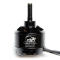
\includegraphics[width=0.9\textwidth]{figs/cobra-motor}
\caption{Cobra CM2208/2000KV BLDC motor}
\label{fig:cobra}
\end{subfigure}
\begin{subfigure}{0.5\textwidth}
\centering
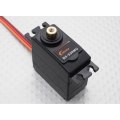
\includegraphics[width=0.9\textwidth]{figs/corona-servo}
\caption{Corona DS-339MG digital servo}
\label{fig:corona}
\end{subfigure}
\caption{}
\end{figure}
Discrete elements for the whole system can potentially limit performance but are going to be mitigated if possible. For example analogue servos have an associated $1 ms$ deadband from their $50 Hz$ refresh rate. That can be addressed by using faster, albeit more expensive, digital servos which samples at $330 Hz$. The prototype's flight controller needs to provide 12 PWM output compare channels for the 8 servos and 4 BLDC speed controllers. State updates from a ground control station and a fail safe 6CH RC receiver module also needs to be processed by the $\mu$C system. Particular attention is paid to the embedded system design and layout in Section:\ref{sec:proto.layout}.%====================================================
\section{Literature Review}
\label{sec:intro.litreview}
%====================================================
\subsection{Existing \& Related Work}
\label{subsec:intro.lit.related}
%====================================================
The field of transformable aerospace frames is not necessarily a new one, with many commercial examples having seen a lot of success over their operational life span. The most notable tilting-rotor vehicle is that of the Boeing/Bell V22 Osprey\cite{.} aircraft. First introduced into the field in 2007, the Osprey has the ability to pitch its two lift propellers forward to aid translational flight after vertically taking off or landing. In addition to this there have been many papers published on similar tilting bi-rotor UAVs for research purposes.
\subsubsection*{Birotors}
\begin{figure}[hbtp]
\centering
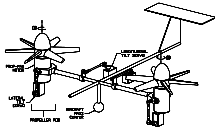
\includegraphics[width=0.8\textwidth]{figs/dualaxistilt}
\caption{General structure for opposed tilting platform}
\label{fig:dualaxistilt}
\end{figure}
Research into birotor vehicles (Fig:\ref{fig:dualaxistilt})\footnote{Image from G. Gress:\cite{gres2007}} with ancilliary lift propeller actuation is oft termed Opposed Active Tilting or \emph{OAT}. Such a rotorcraft's mechanical design applies either a single \emph{oblique} 45\textdegree ~tilting axis relative to the body; \cite{smalltwotilting,obliquepitch,passiveobliquetilting}, or a \emph{lateral} tilting axis, adjacent to the body; \cite{tiltrotorUAV,adaptivebackstep,tiltrotorcontrol,tpheonix}. Leading research is currently focussed on applying doubly actuated tilting axes to birotor UAVs. Dual axis Opposed Active Tilting or \emph{dOAT} introduces vectored thrust with propeller pitch and roll motions to further expand the actuation suite, \cite{gres2007,opposedlateraldualaxis}. A birotor is sometimes considered preferable to higher order multirotor platforms due to their reduced controller effort. However the controller plant abstraction often detracts from the quality and effectiveness of its stability solution as a result of the birotor's underactuation. 
\par
Birotor attitude control typically incorporates plant independent PD \cite{obliquepitch} and PID \cite{tiltrotorUAV} controller schemes. Occasionally more computationally intensive and plant dependent Ideal and Adaptive backstepping controllers (\emph{IBC} or \emph{ABC}) are implemented, presented in \cite{smalltwotilting,tpheonix} and \cite{adaptivebackstep} respectively. The cross-coupling of a birotor vehicle's attitude system is more pronounced than that of a quadrotor, derived in Section:\ref{sec:dynamics.nonlinearities}, and so feedback linearisation is almost always used. In an interesting progression from the norm, Lee et al,  \cite{autopilotPSO}, proposed a PID co-efficient selection algorithm for a bi-rotor control block. Using a Particle Swarm Optimization techinque, similar to \cite{adaptivepso}, the coefficients were globally optimized around a given performance metric. However their performance criterion is a basic ITAE$^\dagger$ term and nothing more appropriate involving effects unique to flight systems. \emph{PSO} algorithms iteratively search for a globally optimized solution and offer independent, derivative free optimization. Later on non-linear controller coefficient are also optimized in this paper using a PSO algorithm, shown in Section:\ref{sec:simulation.tuning}.
\par
\subsubsection*{Quadrotors}
Expanding on multirotor vehicles, the quadrotor UAV is a popular and well researched multirotor platform due to its mechanical simplicity. What would appear to be one of the first quadrotor research implementations, in 2002, is the X4-Flyer quadrotor, \cite{x4flyer,x4flyercontrol}. Alternative iterations like the Microraptor\cite{microraptor} and STARMAC\cite{starmac} quadcopters have subsequently been built and tested. A plethora of literature exists around quadrotor kinematics \& control \cite{dynamicmodelling2013, dynamicmodelling2009, modelingquadcopter, quaddynamics, fullquadcoptercontrol}, however dedicated rigid body 6-DOF dynamic papers \cite{rigidbodylecture,eulerrigidbody} provide better explanations of the kinematics. Often the plant's dynamics are simplified around an origin trim point and assumed to reduce into 6 SISO plants for each degree of freedom (Appendix:\ref{app:stddynamics}). Lately research projects have begun to incorporate aerodynamic effects like drag and propeller BEM theory into the plant model\cite{lowreynolds,bem,starmac}. Although mostly negligible under standard opperating conditions, the higher fidelity models offer more precision without making any linearisations or assumptions,\cite{nonlineardynamics,starmac}.
\par
\begin{figure}[hbtp]
\centering
\begin{subfigure}{.5\textwidth}
\centering
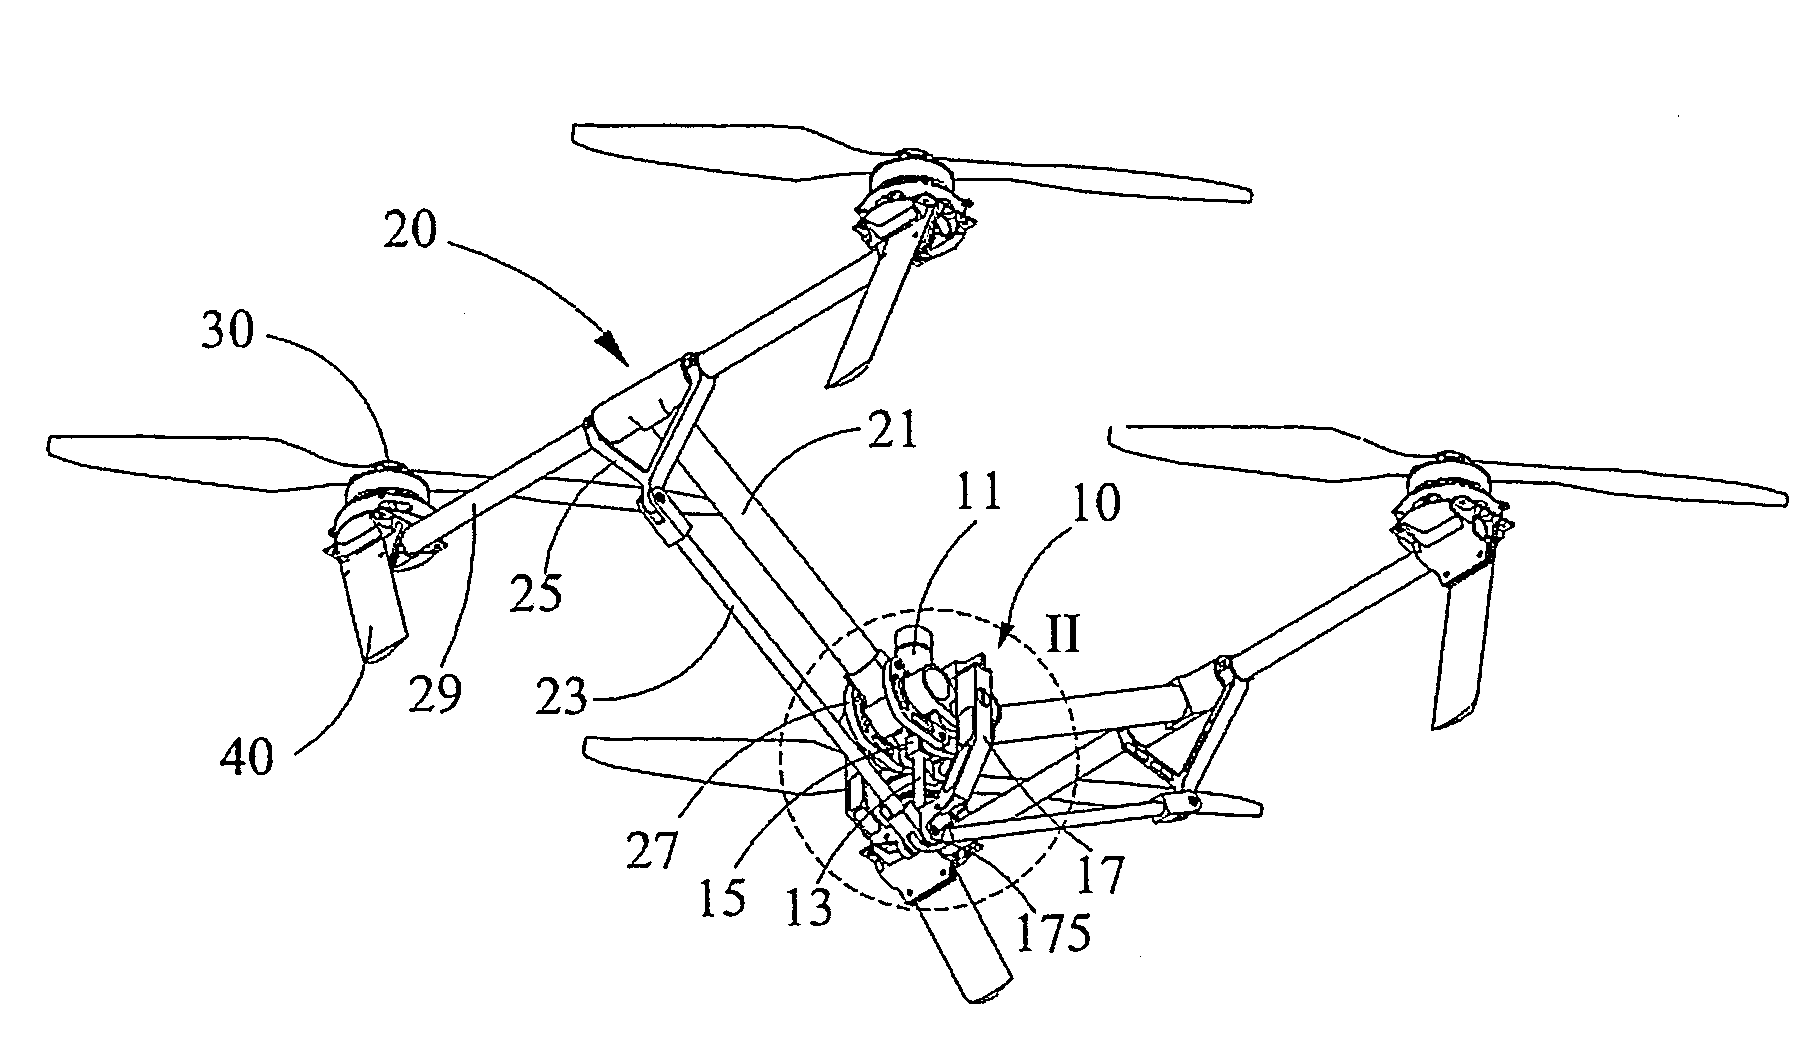
\includegraphics[width=\textwidth]{figs/dji-inspire1}
\caption{Inspire1 articulated upwards}
\label{fig:inspireup}
\end{subfigure}%
\begin{subfigure}{.5\textwidth}
\centering
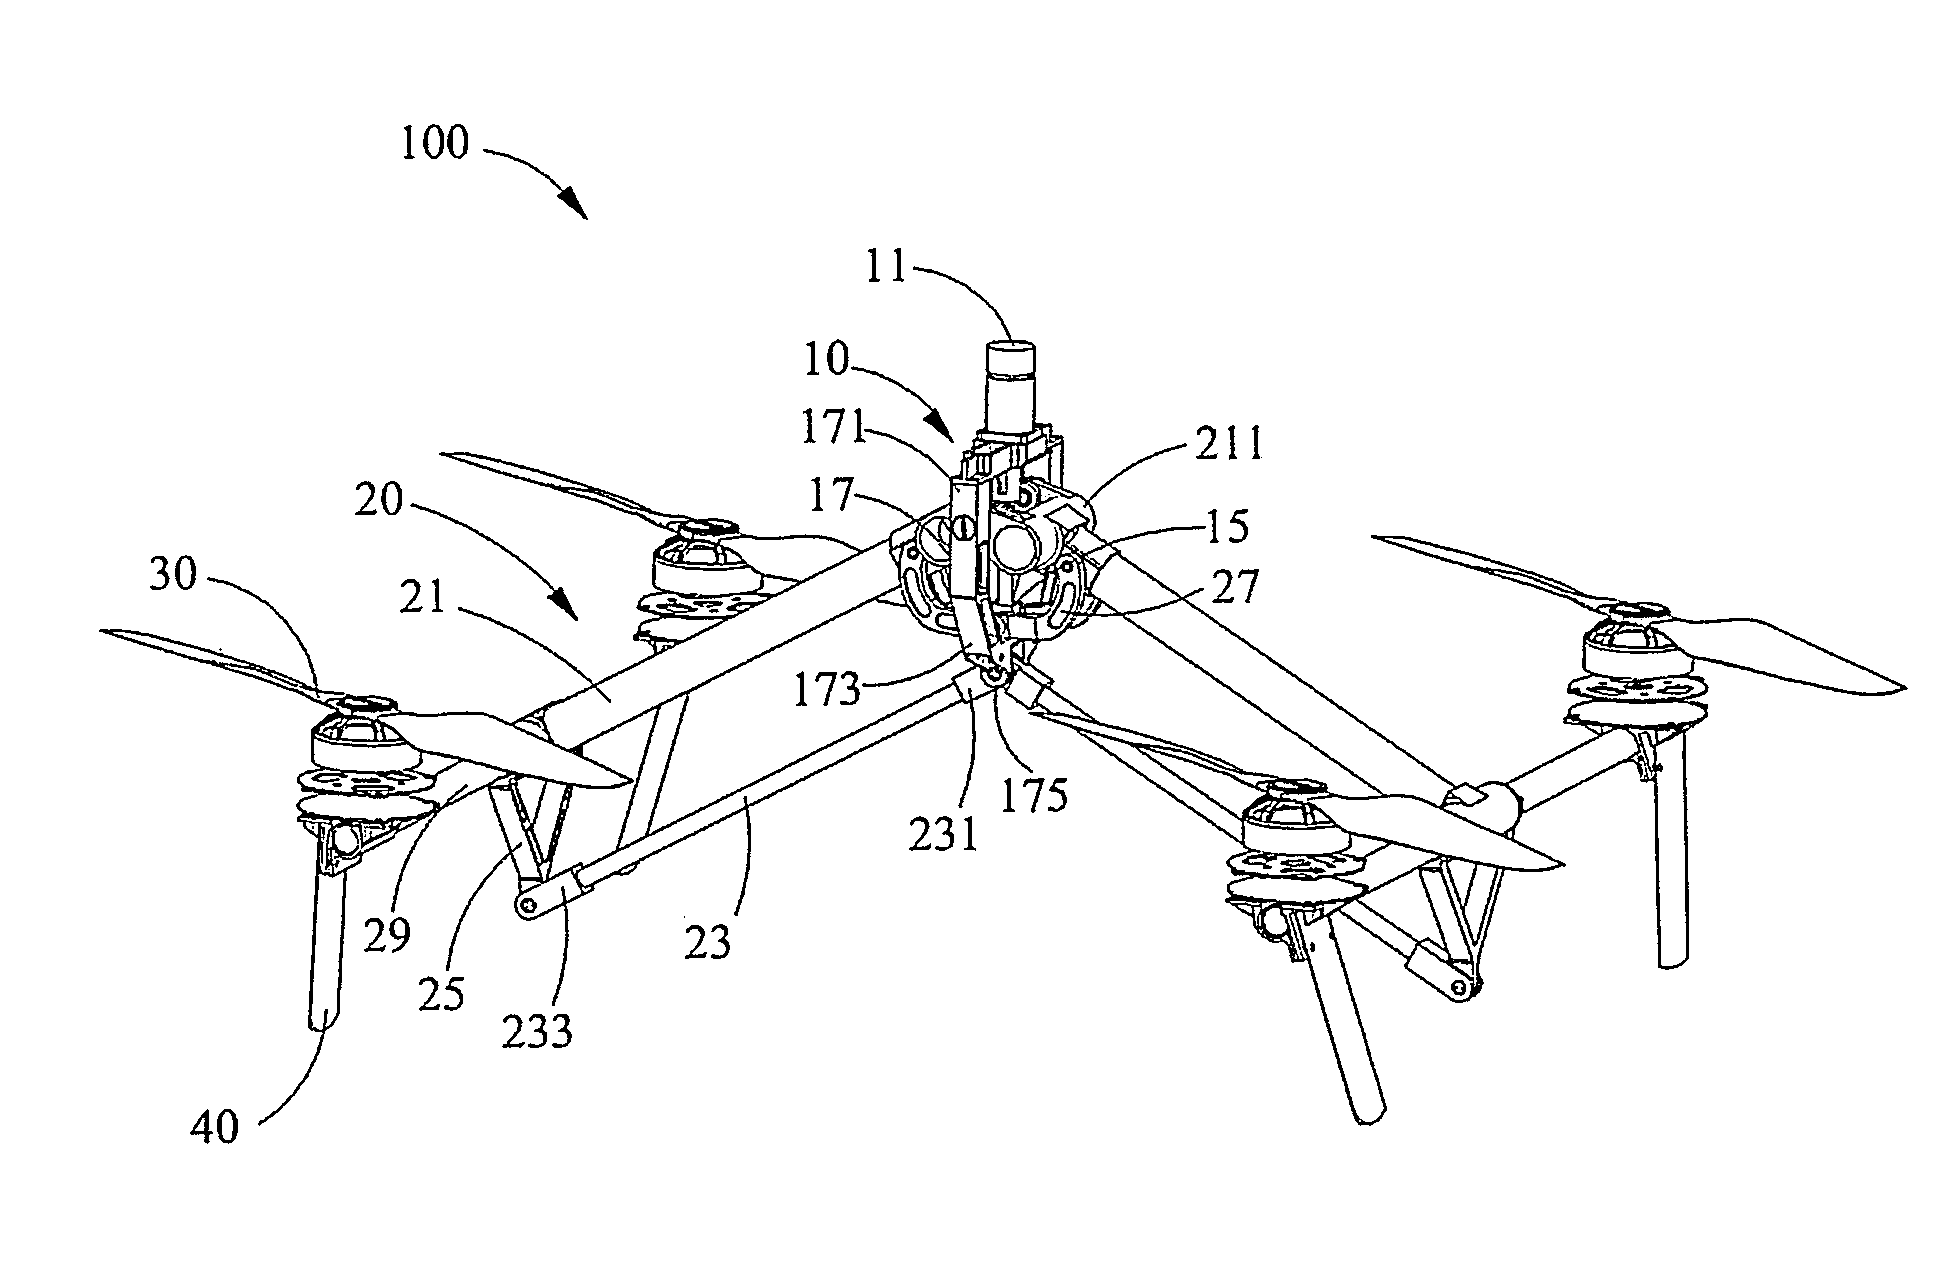
\includegraphics[width=\textwidth]{figs/dji-inspire2}
\caption{Inspire1 articulated downwards}
\label{fig:inspiredown}
\end{subfigure}
\caption{DJI Inspire1}
\label{fig:inspire1}
\end{figure}
At the time of writing, the only commercial UAV multirotor capable of structural transformation is the DJI Inspire1 quadrotor\cite{inspire}, made by Shenzen DJI Technologies (better known for the hugely successful DJI Phantom drone\cite{phantom}). The Inspire1 can articulate its supporting arms up and down as shown in Fig:\ref{fig:inspire1} \footnote{Both images were sourced from the drone's patent, held by SZ DJI Tech Co\cite{djinspire}}. The aim of such movements is to both alter the center of gravity and further expose a belly mounted camera gimbal for panoramic viewing angles. This transformation changes the moment of inertia about the body's center of gravity, in turn changing the inertial torque response induced by angular velocities, an otherwise detrimental effect which makes researchers apprehensive of transformable aerospace frames. The range of transformations which the frame can undergo is limited to just articulating the arms up and down.
\par
In a similar fashion to the progression seen in birotor state-of-the-art, quadrotor research is engaging the topics of single and dual axis tilting articulations. First conceptualized and implemented on a prototype related to an ongoing project covered in two reports, \cite{tiltpropellercontrol,tiltpropellerflight}. The authors M. Ryll et al.(2012, 2013) modified and tested a QuadroXL four rotor helicopter, propduced by MikroKopter \cite{mikrokopter}, to actuate only a single axis of tilting aligned with the frame's arms (Fig:\ref{fig:tiltpropellercontrol1})\footnote{Image sourced from Modelling and Control of a Quadrotor UAV with tilting propellers, \cite{tiltpropellercontrol}}. Their proposed control solution, discussed in detail next in Section:\ref{subsec:intro.lit.control}, assumes no nominal linearised conditions around hover flight, unlike a similar single axis tilting quadrotor prototype designed by Nemati, et al. (2012)\cite{singleaxistilting}. The latter remains  \underline{simulated} but as yet untested.
\par
One approach to improving quadrotor flight response is to alter the manner in which the thrust is mechanically actuated, potentially improving the actuator bandwidth. Drawing from helicopter design, a project by Napsholm, (2013)\cite{napsholm}, purported a quadrotor UAV prototype that used swashplates for varying the propeller pitch and generating torque moments. The aim was a design which wasn't dependent on speed control (\emph{ESC}) power electronics to actuate variable thrust forces. Petrol motors were intended for use in place of BLDC motors. Furthermore, the design proposed a single axis of tilt actuation to each of the four motor modules. Whilst mechanically complex, Napsholm made use of existing RC helicopter components to design a rotor actuation bracket (Fig:\ref{fig:tiltrotor-napsholm}). The cyclic-pitch swashplate used \cite{autonomousrobotspitch} could apply torques, $\tau_{\phi}$ and $\tau_{\theta}$, about each propeller's hub, \emph{principle axis of rotation}, by altering the blades angle of attack throughout its rotational cycle. The actuation rate of such a configuration is far faster than that of a differential torque produced rolling/pitching motion.
\begin{figure}[htbp]
\centering
\begin{subfigure}{.5\textwidth}
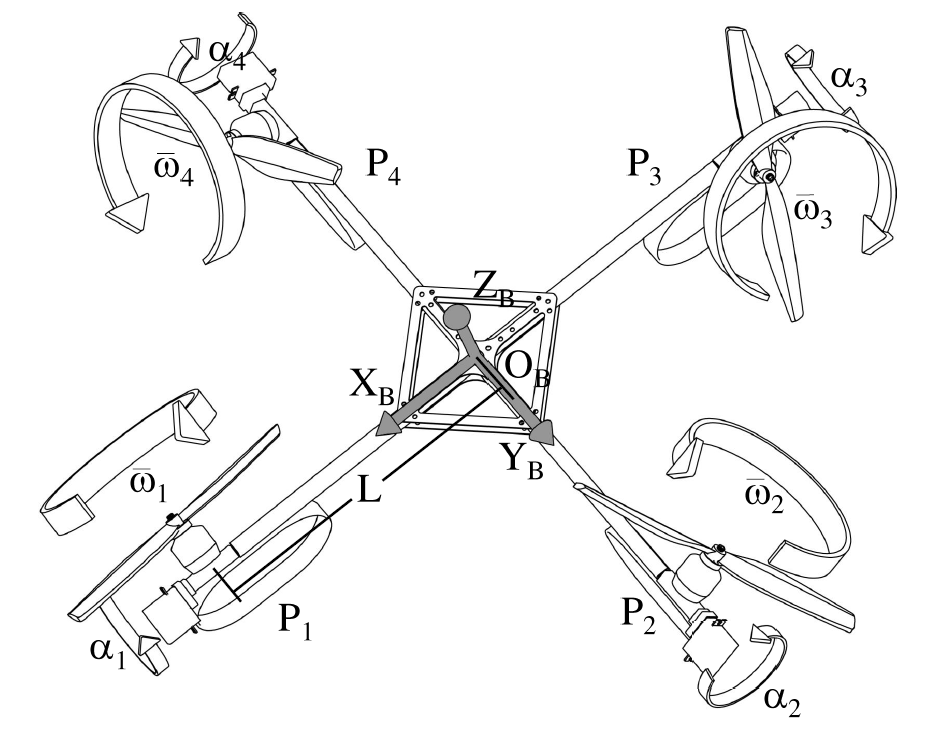
\includegraphics[width=\textwidth]{figs/tiltpropellercontrol1}
\caption{Single rotation axis aligned with the frames arm}
\label{fig:tiltpropellercontrol1}
\end{subfigure}%
\begin{subfigure}{.5\textwidth}
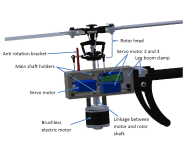
\includegraphics[width=\textwidth]{figs/napsholm-mech}
\caption{Cyclic-pitch \& swashplate mechanism}
\label{fig:tiltrotor-napsholm}
\end{subfigure}
\caption{}
\label{fig:tiltprop}
\end{figure}
\par
Irrespective of the strong initial design in the early stages of his project, it would appear that Napsholm's research suffered due to time constraints. The introductory derivation on aerodynamic effects and deliberation over the design provide clear insight into the projects goals. However the control solution and system architecture, electronic and software, are significantly lacking. An introductory proposal of an MPC attitude control system detracted from the comprehensive dynamics discussed. The project ended before testing, simulation and results could be obtained. Unfortunately, despite the novel over-actuated design, there was no discussion given on how the allocation, being the most unique aspect, would be achieved.
\par
Finally, the most crucial research to mention is a project completed by Pau Segui Gasco \cite{tiltgasco}, which was a dual presented MSc project with Yazan Al-Rihani \cite{tiltrihani}. At the time of writing, this would appear to be the only project published pertaining to \emph{over-actuation} in aerospace bodies implemented on a quadrotor platform. The research was split between the two authors who completed the control/electronic design and the mechanical design for their respective MSc dissertations. Shown in Fig:\ref{fig:tiltrotor-gasco}\footnote{Image from Development of a Dual Axis Tilt Rotorcraft UAV: Modelling, Simulation and Control \cite{tiltgasco}}, the dual-axis articulation is achieved using an RC helicopter tail bracket and servo push-rod mechanism; reducing the mass of the articulated component but limiting the range of its actuation. Considering the propellers as a spinning flywheel, the induced gyroscopic response was then be treated as a controllable actuator plant. Their commanded virtual control is distributed by weighted inversion among the actuator set, Section: \ref{subsec:intro.lit.control}. The whole project justifies the extra actuation as fault tolerance redundancy but doesn't necessarily prove how such a redundancy could be beneficial.
\begin{figure}[htbp]
\centering
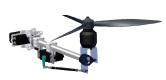
\includegraphics[width=0.7\textwidth]{figs/gasco-mech}
\caption{Dual-axis tilt-rotor mechanism}
\label{fig:tiltrotor-gasco}
\end{figure}
%====================================================
\subsection{Notable Quadrotor Control Implementations}
\label{subsec:intro.lit.control}
%====================================================
\subsubsection*{Quadcopter Attitude Control}
%====================================================
Attitude control of a 6-DOF body is best described by \emph{The Attitude Control Problem} \cite{attitudecontrolproblem}. A rigid body that currently has an attitude state\footnote{Quaternion attitude states will later replace Euler angles} $\vec{\eta}_s$ and a desired state $\vec{\eta}_d$, the problem is to then find a torque control law:
\begin{equation} \label{eq:2}
\mu\tau = H(\vec{\eta}_s,\vec{\eta}_d,\dot{\vec{\eta}}_s,\dot{\vec{\eta}}_d)
\end{equation}
Such that both the angular position $lim~\vec{\eta}_s \rightarrow \vec{\eta}_d$ and that angular rates $lim~\dot{\vec{\eta}}_s \rightarrow \dot{\vec{\eta}}_d$ asymptotically stabilize as $t \rightarrow \infty$. A distinction must be made between angular rate vector, $\dot{\vec{\eta}}=[\dot{\phi}~\dot{\theta}~\dot{\psi}]^T$ and the angular velocity vector $\vec{\omega}_b=[p~q~r]^T$. Depending on how the attitude is posed; with rotation matrices \cite{rigidbodylecture,eulerrigidbody,rotationsequences}, quaternions \cite{quaterniondynamics, rotationsequences, spacecraftattitutdequaternions,fullquaternion} or otherwise (Direct Cosine Matrix etc \ldots) the error sate\footnote{\emph{The Attitude Control} \cite{attitudecontrolproblem} describes these conventionally different error states} $\Delta\vec{E}= \vec{\eta}_d - \vec{\eta}_s$ could then differ to a (hamilton) multiplicative relationship.
\\
\emph{\color{Gray}Note that here $\vec{\eta}$ is not necessarily an Euler set but any attitude representative state variable.}
\par
Simulation and modelling papers often rely on Euler angle based rotation matrices for attitude representation, \cite{adaptivedisturbancecontrol, optimizedpidquadcopter, singleaxistilting, backsteppingquadcoptercontrol, fullquadcoptercontrol} without addressing the inherent singularity associated with such an attitude representation (sic Gimbal Lock, \cite{euleranglesingularity}, Section:\ref{subsec:dynamics.rigidbody.singularity}). The alternative quaternion attitude representation, first implemented on a quadrotor UAV in 2006 \cite{attitudestabilization}, is often used in lieu of rotation matrices but has its own caveat of \emph{unwinding}, (Section:\ref{subsec:dynamics.rigidbody.unwinding}), as a result of quaternions dual-coverage \cite{unwinding} in $\mathbb{R}^3$ space. Quaternions are $\in\mathbb{R}^4$ variables for attitude representations and so a mapping $\rightarrow\mathbb{R}^3$ produces a dual coverage for each attitude state.
\par
Quadrotor plant dynamics, as mentioned previously, are often simplified; especially when represented with a 3-variable Euler angle set, $\vec{\eta} = [\phi ~\theta ~\psi]^T$. The coupled gyroscopic and Coriolis responses are both neglected when the angular velocity\footnote{Angular velocity and angular rates are fundamentally different, $\vec{\omega}_b\not=\dot{\vec{\eta}}$} is small, $\vec{\omega}_b \approx 0$, and the inertial matrix is diagonal, $rk(\mathbb{I}_f)= x$ for $\in\mathbb{R}^x$. The consequence of which is the ineffectual deterioration of both the gyroscopic term, $\vec{\tau}_{gyro}=-\vec{\omega}_b \times \mathbb{I}_b\vec{\omega}_b \approx 0$ and the  Coriolis force term, $\vec{F}_{cor}=-\vec{\omega}_b \times \vec{a_b} \approx 0$ in the bodies dynamics~~(Chapter:\ref{ch:dynamics} for context). Once the coupled cross-product terms are no longer of consequence, the 6 DOF, $[x ~y ~z ~\phi ~\theta ~\psi]^T$, can be treated as a series of individual SISO plants each controlled with an appropriate technique. Quaternion represented attitude plants cannot easily be decomposed into individual single-input-single-output systems (quaternion dynamics in Section:\ref{subsec:dynamics.rigidbody.quaternion}). So a quaternion (combined four variable attitude state vector) is then used, $Q_b = [q_0 ~\vec{q}\>]^T$ for the abstracted major loop plant.
\par
\begin{figure}[hbtp]
\centering
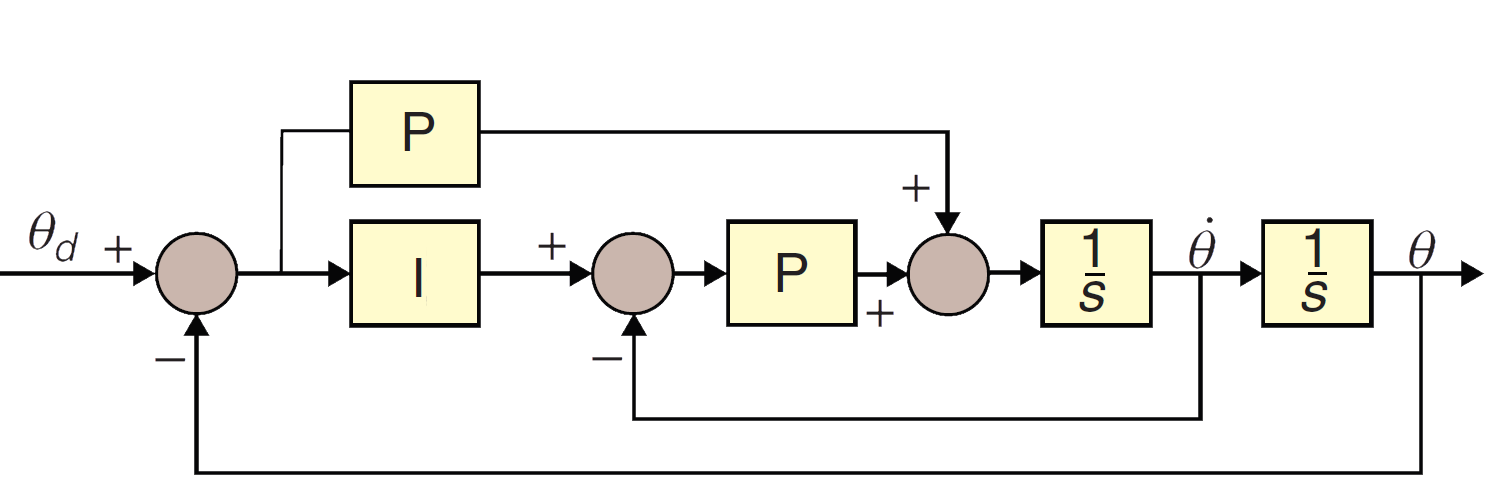
\includegraphics[width=0.8\textwidth]{figs/arducopter-pi}
\caption{ArduCopter PI Euler angle attitude control loop}
\label{fig:arducopter-pi}
\end{figure}
Commercial flight controllers' software (Arducopter\cite{arducoptersite}, Openpilot\cite{openpilotsite}\footnote{\underline{NOTE:} OpenPilot's firmware stack is now maintained by LibrePilot}, CleanFlight\cite{cleanflight}, BetaFlight\cite{betaflight}, etc \ldots) for custom fabricated UAV platforms all apply their own flavour of structured attitude controllers and state estimation algorithms, based on onboard hardware sensor fusion. The article \emph{Build Your Own Quadrotor}\cite{buildyourownquad} summarizes the control structures implemented on a range of popular flight controllers. The most popular of which, ArduCopter, implements a feed-forward PI compensation controller (Fig:\ref{fig:arducopter-pi})\footnote{Image sourced from \emph{Build your own Quadrotor}\cite{buildyourownquad}}.  PI, PD and PID controllers are all easy and effective plant independent control solutions for general attitude plants. Table:\ref{tab:controllers} collectively lists the common attitude control blocks (not exclusively quadrotors UAVs but MAVs too) and which projects they've been implemented in, after which a critique on the more unique adaptations is given.
\begin{table}[h]
\centering
\begin{tabular}{ |c|l|l|c| }
\hline
Controller Type & Independent & Dependent & Total\\ \hline
PI & \cite{attitudecontrolproblem} & \cite{attitudecontrolproblem} & 2\\ \hline
PD & \cite{modelingquadcopter, tiltrihani} & \cite{fullquaternion,singleaxistilting} & 4\\ \hline
PID & \cite{optimizedpidquadcopter, attitudecontrolproblem, quaddynamics, tiltpropellercontrol, pidlqr} & \cite{attitudecontrolproblem, starmac, adaptivedisturbancecontrol} & 8\\ \hline
Lead & \cite{x4flyer, dynamicmodelling2009} & lead & 2\\ \hline
IBC & \cite{tpheonix, backsteppingquadcoptercontrol}\footnote{\cite{tpheonix} applied an IBC algorithm derived through Hurwitz polynomials, not lyupanov theorem.} & \cite{backsteppingquadcoptercontrol} & 3\\ \hline
ABC & \multicolumn{2}{l|}{\cite{adaptivebackstep, nonlinearadaptive, 6dofbackstep, intelligentbackstep}} & 4\\ \hline
LQR & \cite{pidlqr} & LQR & 1\\ \hline
\end{tabular}
\caption{A breakdown of common attitude controllers}
\label{tab:controllers}
\end{table}
\par
In a collection of papers, written by Bouabdallah et al \ldots (2003,2004,2007) arguably the most prolific early quadrotor authors, a range of different control implementations are derived and reviewed. Their last paper (2007)\cite{fullquadcoptercontrol} derived and pratically tested an Integral Backstepping attitude controller on an OS4 quadrotor platform. It builds on their research from an earlier paper (2003)\cite{pidlqr} wherein an analysis of PID vs LQR attitude controllers in the context of quadrotors is posed. LQR controllers aim to optimize the controller effort (with $u\in\mathbb{U}$, controller effort is then $||u||$ or the $L_2$ norm of the plant input). Although, in theory, solving the assocaited Ricatti$^{\dagger}$ cost function may produce an optimial, stable and efficient control law it needs exact plant matching. In practice, exact plant matching is difficult to achieve for a quadcopter or any aerospace body for that matter. The resultant controller in \cite{pidlqr} achieved asymptotic stability but had poor steady state performance due to low accuracy of the identified actuator dynamics and poor inertial measurements.
\par
Adaptive Backstepping Control\cite{backstepping}(any of the examples in Table:\ref{tab:controllers}) builds on nominal IBC fundamentals by introducing an aditional disturbance state term in the LCF used for the backstepping iteration. The drawback with this form of Backstepping approach is that, from the Lyupanov control theorem, a time derivative for the estimated disturbance (or an \emph{update law}) is needed. Disturbance approximation has been investigated thoroughly but, for a signal without \emph{apriori} information, some heuristic needs to be adopted with the approximation which usually involves some compromise.
\newpage
In one example, \cite{nonlinearadaptive}, the authors implemented a statistical $proj(.)$ operator based technique. Which, when used in adaptive control, the projection operator \cite{outputfeedback}, $proj(.)$, ensures a derivative based estimator is bounded for adaptive regression approxmation \cite{nonlinearregression}.
\par
Although the control implementation isn't backstepping based, in \cite{adaptiveslidingmode}, a sliding mode controller was used to compensate for the disturbances in an Unmanned Submersible Vehicle atttiude plant. The underwater current disturbances were approximated using a fuzzy logic system, specifically a \emph{zero-order TSK} fuzzy controller. The TSK system has been proven to act in the same way as an Artificial Neural Network approximator\cite{zeroTSK}; where the TSK system is more comprehensible than the latter. Statistical analysis and investigation of approximators without \emph{apriori} knowledge of a system are well beyond the scope of this research
 but are worth mentioning.
%====================================================
\subsubsection*{Single/Dual Axis Control \& Allocation}
%====================================================
The extra actuation introduced with single and dual axis articulation provides room for more control goals to be achieved as the order of actuation increases. Of the few papers published on tilting-axis quadrotors, PD controllers (Nemati et al.[2014]\cite{singleaxistilting} and again in Gasco \& Rihani \cite{tiltgasco,tiltrihani}) and PID controllers (Ryll et al.[2012,2013]\cite{tiltpropellercontrol,tiltpropellerflight}) are the norm for control blocks. For either of these systems there needs to be an allocation rule to distribute a commanded input amongst the actuator set. In \cite{allocation}, Johansen et al.[2012] describes the control allocation problem for a dynamic plant:
\begin{subequations} 
\begin{equation} \label{eq:3.1}
\dot{x}=f(x,t)+g(x,t)\tau
\end{equation}
\vspace{-20pt}
\begin{equation} \label{eq:3.2}
y=l(x,t)
\end{equation}
\end{subequations}
\emph{\color{Gray} Note in state space Equation:\ref{eq:3.1}, it's assumed the plant input\footnote{Disambiguation: $\tau$ is not necessarily the torque input.}, $\tau$, has a linear multiplicative relationship with the input response, $g(x,t,\tau)\iff g(x,t)\tau$.}
\\
With a state $x\in \mathbb{R}^n$ and $f(x,t)$ \& $g(x,t)$ being the plant's dynamics and input response respectively. In set point tracking, the output is then \emph{tracking} the state $y = x$, and hence $y \in \mathbb{R}^n$. In an ideal well posed system the number of actuator inputs equals the number of controllable variable outputs; that being $dim(x)=dim(\tau)\in \mathbb{R}^n$. In the case where the control input $\tau \in \mathbb{R}^m$, if $m>n$ the problem is then overactuated and a level of abstraction is needed; an asymptotically stabilizing virtual control input $\nu_d$ is designed by a control law $\nu_d=h(x_e,t)$ to affect dynamics. The goal is to then find a function that maps $\mathbb{R}^m \rightarrow \mathbb{R}^n$ for an actuator matrix $u \in \mathbb{U}^m$. An overactuated plant can be described in state-space as:
\begin{subequations}
\begin{equation} \label{eq:3.3}
\dot{x}=f(x,t)+g(x,t)\nu_d,~\nu_d \in \mathbb{R}^n
\end{equation}
\vspace{-20pt}
\begin{equation} \label{eq:3.4}
\nu_c=B(x,t,u)\approx B(x,t)u, ~u\in \mathbb{U}^m,~\nu_c\in\mathbb{R}^n
\end{equation}
\vspace{-20pt}
\begin{equation}
y=x
\end{equation}
\end{subequations}
$B(x,t,u)$ is the effectiveness function which quantifies how the actuator inputs $u$ relate to the virtual commanded input $\nu_c$. $B(x,t,u)$ can be abstracted to a multiplicative relationship $B(x,t)u$ if the plant's dynamics permit it, such that; $B(x,t)\in\mathbb{R}^{n\times m}$. For generic setpoint tracking the control law will design a desired virtual control input $\nu_d$, the allocation rule then has to solve $u$ for $\nu_c$ such that a slack variable $s=\nu_c-\nu_d$ is minimized:
\begin{equation}\label{eq:quadraticallocator}
\underset{u \in \mathbb{R}^m ,s \in \mathbb{R}^n}{min}\norm{Q_s} ~\text{subject to} ~B(x,t,u) - h(x_e,t)=\nu_c-\nu_d=s,~u \in \mathbb{U}
\end{equation}
Which ensures the commanded input $\nu_c$ tracks the desired control input $\nu_d$; $\nu_c\rightarrow\nu_d$ as per some cost function of the slack variable $Q_s$. Mostly the L2 norm, $\norm{Q_s}$, is used. In an overactuated system it then follows that there is a set of possible inputs for each $\nu_c$. A unique actuator solution (rather than a family solution set) to Eq:\ref{eq:quadraticallocator} needs a secondary objective function, $J(x,t,u)$. Eq:\ref{eq:quadraticallocator} then becomes;
\begin{equation} \label{eq:quadraticallocatorcost}
\underset{u \in \mathbb{R}^m ,s \in \mathbb{R}^n}{min}(\norm{Q_s}+J(x,t,u)) ~\text{subject to} ~\nu_c - h(x_e,t)=s, u \in \mathbb{U}
\end{equation}
\newpage
Those same authors Johansen and Tjønnås [2004,2005,2008] proposed multiple control allocation solutions to a variety of systems. Following \cite{allocation}, in a subsequent paper \cite{efficientallocation}, Johansen and Tjønnås [2005] introduce a secondary cost function, driving the solution away from the typical quadratic programming direct or weighted inversion solution. Aiming for optimal efficiency and not just actuator saturation. In a followup paper\cite{adaptiveallocation}, the same authors proposed an online adaptive algorithm approach, using a Lyupanov energy function, to ensure the minimization adaptive law settles to a feasible solution.
\par
Over-actuation is not something often applied to quadrotors and as a result rather than providing a comprehensive literature review of associated papers here (which are all mostly theoretical derivation), the contextual application and solutions to the above posed problems are expanded later in Section:\ref{subsec:control.allocation.allocators}. The only overactuated quadrotor (birotor dual-axis tilting makes the system critically actuated and so requires no allocation) literature which covers allocation of the extra actuators is \cite{tiltgasco,tiltrihani}, where the authors apply a weighted pseudo inverse (sic Moore Penrose Inverse \cite{moorepenrose}) allocation rule. A prerequisite for pseudo inversion is a multiplicative \emph{linear} control effectiveness relationship for Eq:\ref{eq:3.4}. 
\par
Segui et al. [2012] applied weighted inversion, relying on some very specific assumptions to achieve that linearity relationship in Eq:\ref{eq:3.4}. For the net torque response the authors assumed the extra actuators pitch and roll angular rates, $\dot{\phi}$~and~$\dot{\theta}$ respectively, were proportionally related as follows:
\begin{equation}
\dot{\phi}\approx\frac{\phi}{t_{rise}}
\end{equation}
In which $t_{rise}$ is the actuators rise time to a set-point. As a result the gyroscopic first order torque $\tau_{gyro}=-\omega\times\mathbb{I}_f\omega$ and second order inertial torque $\tau=\mathbb{I}\dot{\omega}$ are then functions of position $\phi$ or $\theta$ and not their derivatives. The extent of that consequence is contrasted with the allocation solution in Section:\ref{sec:control.allocation}.
%====================================================
\subsubsection*{Satellite Attitude Control}
%====================================================
Unconstrained attitude set-point tracking for 6-DOF bodies, quaternion represented or otherwise, is a topic well covered in the field of satellite attitude control; \cite{axissymmetricspacecraft, satellitebackstepping,lpvbackstepping}. The \emph{status quo} for recent research is on non-linear adaptive attitude back-stepping control systems, wherein the adaptive update rule is the novel contribution. Often plant uncertainty affects the inertial tensor of a satellite. In \cite{lpvbackstepping}, the authors Wang Jia, et al. [2010], proposed applying adaptive back-stepping to compensate for steady state errors of (asymmetric) inertial estimations. Alternatively, instead of deliberating on costly non-orbital prelaunch inertial measurements Bodrany, et al.[2000]\cite{inertiaestimation} developed an algorithm for estimating the inertia tensor based on controlled single axis perturbations. Such an approach does assume any initial estimates are sufficiently close to true body values such that they will settle and stability can be ensured, irrespective of how unacceptable the transient performance may be.
\par
Satellite actuator suites mostly include additional redundant effectors, to ensure fault tollerance, and thus require control allocation. Often the extra allocators are CMG actuators, driven by DC motors, to produce rotational torques. Fuel burning can only actuate for a certain period of time and so thrusters are scheduled to have a lower priority. Seen in the paper \cite{satellitebackstepping}; the authors, Kristiansen et al. [2005], address the over-actuation with direct and well-matched inversion before applying quaternion based back-stepping for attitude control. A direct inversion solves to Eq:\ref{eq:quadraticallocatorcost} such that:
\begin{subequations}\label{eq:pseudoinv}
\begin{equation}\label{eq:pseudoinva}
u=B^{\dagger}({\tau_a}^{b}-D{\omega_{ib}}^b)
\end{equation}
\vspace{-15pt}
\begin{equation}\label{eq:pseudoinvb}
B^\dagger=B^T(BB^T)^{-1}
\end{equation}
\end{subequations}
Where $B$ is the effectiveness matrix and $B^{\dagger}$ is such that $BB^{\dagger}=\mathbb{I}$. Specifically $B^{\dagger}$ is the general \emph{pseudo} inverse of $B$ (more on inversions in Sec:\ref{sec:control.allocation}). It's assumed there's a multiplicative relationship between the input, $u\in\mathbb{U}$, and the input effectiveness matrix in Eq:\ref{eq:3.4}. The controller designed actuator torque ${\tau_a}^b$ then dictates the input $u$ as in Eq:\ref{eq:pseudoinva}. Much like the over-actuation previously discussed W.R.T quadcopters; the pseudo inversion method of actuator distribution applies quadratic optimization to the allocation slack cost function, Eq:\ref{eq:quadraticallocator}. 